\documentclass[11pt,a4paper]{article} 
\usepackage[portuges]{babel}
\usepackage[utf8]{inputenc}
\usepackage{graphicx}
\usepackage{listings}
%\renewcommand{\lstlistingname}{Algoritmo} 
\usepackage{amsthm}
\usepackage{booktabs}
\usepackage{amsfonts}
\usepackage{subcaption}
\newtheorem{lema}{Lema}
\newtheorem{corolario}{Corolario}
\newtheorem{teorema}{Teorema}
\graphicspath{{images//}}

\title{Relatório - Trabalho 1 \\ Algoritmos de ordenação}
\author{Ronald A. Kaiser}


\begin{document}
    \maketitle

    \paragraph{}
    Para este trabalho, implementamos e analisamos o desempenho de 5 algoritmos de ordenação apresentados em sala de aula: selection sort, insertion sort, merge sort, quick sort e heap sort. Testamos o desempenho dos algoritmos para diversos tipos de entrada númericas e ainda os adaptamos para ordenar palavras.

    \section{Implementação}
        \paragraph{}
        Vamos inicialmente fazer uma breve análise do esforço envolvido na implementação dos algoritmos.


        \subsection{Selection Sort}
            \paragraph{}
            Indubitavelmente, o algoritmo de mais fácil implementação dentre todos.
            \paragraph {}
            Selection sort percorre sistematicamente o array procurando o menor elemento a cada interação. Por essa característica, sua implementação não requer que se pense em exceções, nem em chamadas recursivas. Como visto em aula, o algoritmo não se adapta à entrada. Assim, o número de comparações só depende do \textbf{tamanho} da entrada e não de sua \textbf{qualidade}. 
            

        \subsection{Insertion Sort}
        \paragraph{}
        A ideia principal do algoritmo é equivalente ao procedimento usado para ordenar cartas de uma mão de baralho. A cada nova carta adicionada, procuramos seu lugar dentre as cartas previamente ordenadas. Assim, dependendo da configuração das outras cartas o número de comparações pode ser diferente para entradas distintas. Esse "procurar o lugar certo" para a nova carta torna o algoritmo adaptável à entrada e por isso, sutilmente mais complicado de implementar do que o Selection Sort.


        \subsection{Merge Sort}

        \paragraph{}
        A ideia principal do Merge Sort é \textbf{dividir} o problema inicial em dois subproblemas com a metade do tamanho cada um e uma vez resolvidos os subproblemas, combinamos as soluções para \textbf{conquistar} o problema inicial. 
        \paragraph{}
        A ideia de dividir o problema inicial em subproblemas comumente se aproveita de chamadas recursivas. Orquestrar as chamadas recursivas de tal modo exige um pouco mais de cuidado na implementação e por esse motivo, o Merge Sort se torna mais custoso de se implementar do que o Selection Sort e o Insertion Sort.
        

        \subsection{Quick Sort}
        \paragraph{}
        Assim como o Merge Sort, o Quick Sort possui uma abordagem de divisão e conquista. Sua estratégia é escolher um pivô e dividir o problema inicial em dois: um com valores menores do que o pivô e outro com valores maiores do que o pivô. Após a divisão, resolvemos recursivamente os problemas menores sem o pivô. Administrar essas divisões torna o Quick Sort mais difícil de implementar do que o Selection Sort e Insertion Sort. 

        \paragraph{}
        Diferentemente do Merge Sort, o Quick Sort possui uma complicação adicional para a escolha do pivô. Uma escolha errada de pivô pode fazer com que o algoritmo tenha um desempenho bem inferior aos outros (pior caso). Usando um pivô sempre no final da sequência de uma entrada ordenada de modo decrescente o tempo do Quick Sort é bastante prejudicado, pois os subproblemas não são divididos de forma balanceada. Este relatório acompanha uma implementação que gera este comportamento e outra com o pivô sendo escolhido aleatoriamente.


        \subsection{Heap Sort}
        \paragraph{}
        Dentre todos os algoritmos brevemente descritos, o Heap Sort é o primeiro que introduz uma nova estrutura de dados para resolver o problema de ordenação. A manutenção da heap torna o algoritmo mais complicado de implementar do que o Selection Sort, Insertion Sort e Merge Sort.  
        \paragraph{}


    \section{Desempenho}
        \paragraph{}
        Para testar o desempenho dos algoritmos implementados foram usados diversos tipos de entrada. Abaixo, você pode ver os gráficos obtidos. A seguir, faremos considerações sobre eles.

\begin{figure}[]
  \begin{center}
      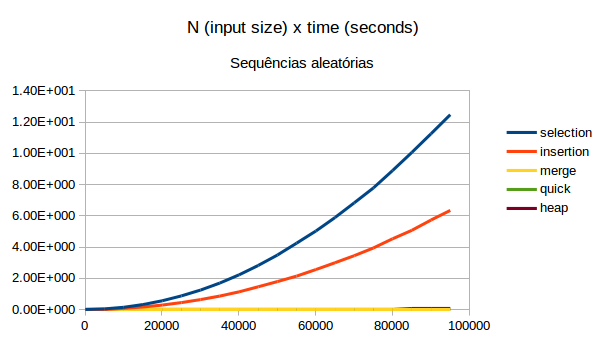
\includegraphics[width=1\textwidth]{random}
  \end{center}
      \label{fig:a}
\end{figure}

\begin{figure}[]
  \begin{center}
      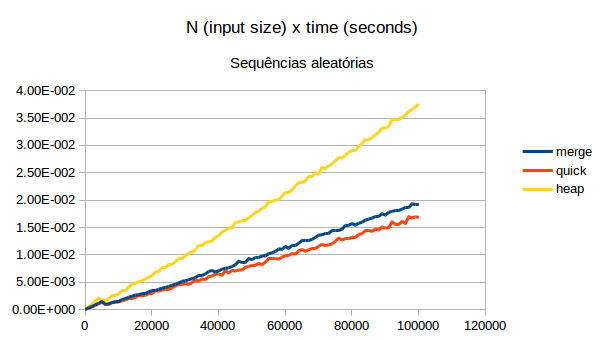
\includegraphics[width=1\textwidth]{random_nlogn}
  \end{center}
      \label{fig:b}
\end{figure}

\begin{figure}[]
  \begin{center}
      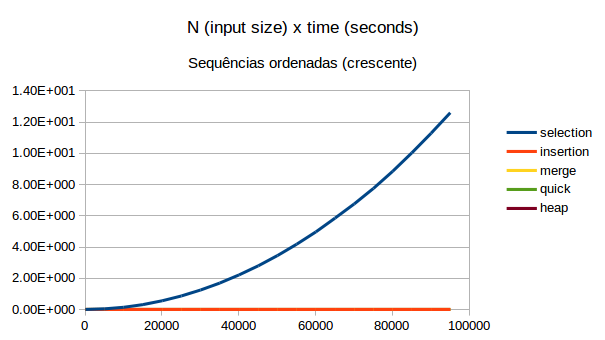
\includegraphics[width=1\textwidth]{sorted_up}
  \end{center}
      \label{fig:c}
\end{figure}

\begin{figure}[]
  \begin{center}
      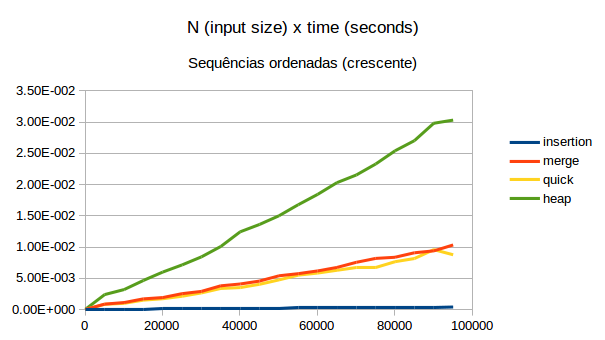
\includegraphics[width=1\textwidth]{sorted_up_zoom}
  \end{center}
      \label{fig:d}
\end{figure}

\begin{figure}[]
  \begin{center}
      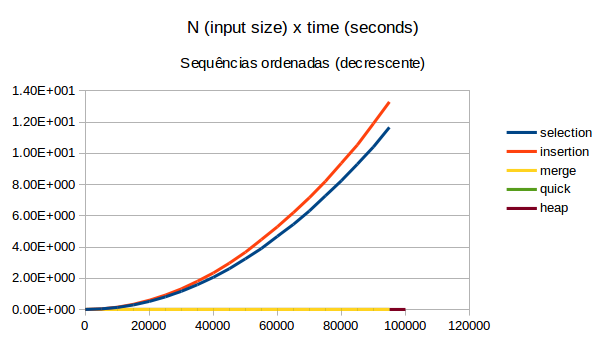
\includegraphics[width=1\textwidth]{sorted_down}
  \end{center}
      \label{fig:e}
\end{figure}


\begin{figure}[]
  \begin{center}
      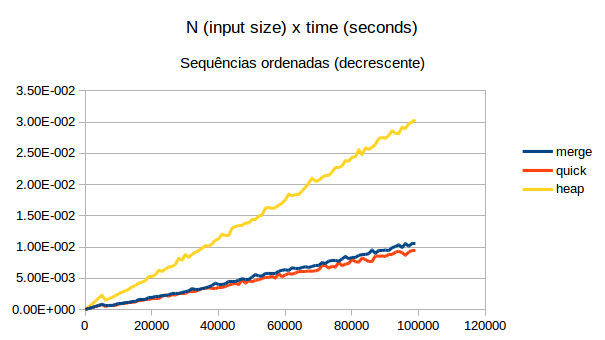
\includegraphics[width=1\textwidth]{sorted_down_zoom}
  \end{center}
      \label{fig:f}
\end{figure}

\begin{figure}[]
  \begin{center}
      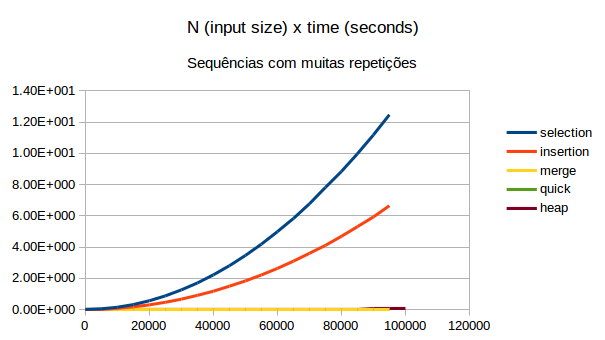
\includegraphics[width=1\textwidth]{lotrept}
  \end{center}
      \label{fig:g}
\end{figure}

\begin{figure}[]
  \begin{center}
      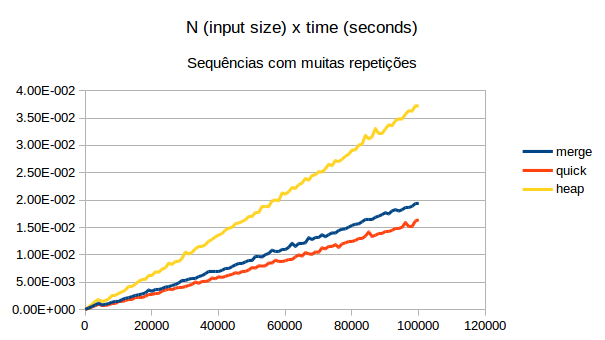
\includegraphics[width=1\textwidth]{lotrept_zoom}
  \end{center}
      \label{fig:h}
\end{figure}

\begin{figure}[]
  \begin{center}
      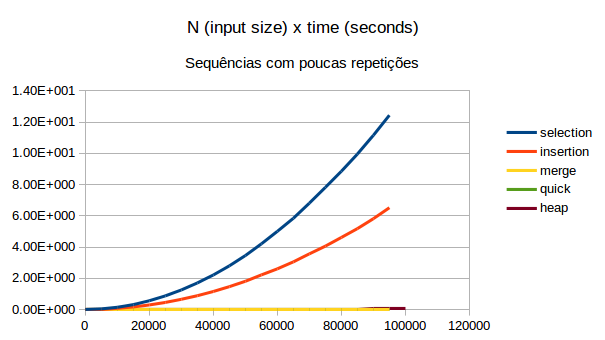
\includegraphics[width=1\textwidth]{fewrept}
  \end{center}
      \label{fig:i}
\end{figure}

\begin{figure}[]
  \begin{center}
      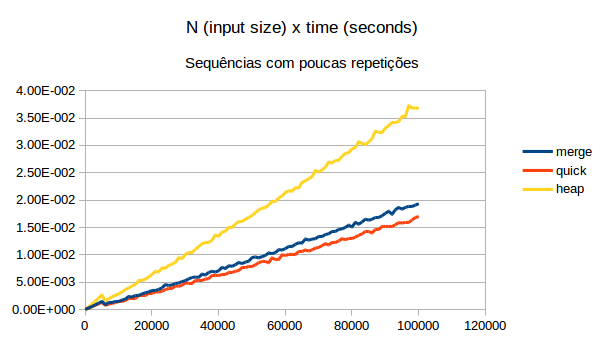
\includegraphics[width=1\textwidth]{fewrept_zoom}
  \end{center}
      \label{fig:j}
\end{figure}

    \paragraph{}
    Dos gráficos obtidos é possível observar que na maioria dos casos o Quick Sort se demonstrou superior aos outros algoritmos. Em contrapartida, o Selection Sort teve o mesmo desempenho para todo tipo de entrada, com o pior tempo de execução dentre os 5 algoritmos. 
    \paragraph{}
    É possível perceber também que os tempos de Heap Sort, Merge Sort e Quick Sort são parecidos, com Heap Sort $>$ Merge Sort $>$ Quick Sort, em geral. Por esse motivo, foi gerado para cada tipo de entradas um gráfico extra para observarmos melhor seus desempenhos. Importante também notar que o Insertion Sort ganha a disputa pelo melhor tempo quando as entradas estão ordenadas de modo crescente, caso em que Insertion Sort tem complexidade O(n).

    \section{Otimizando merge sort e quick sort}
    \paragraph{}
    Afim de melhorar ainda mais o desempenho do Merge Sort e Quick Sort foram implementadas versões híbridas destes algoritmos com o Insertion Sort. A ideia é executar o Insertion Sort quando o subproblema for pequeno o suficiente. Para descobrirmos um valor aproximado para o Threshold, executamos o Insertion Sort, Merge Sort e Quick Sort para as mesmas entradas com o pior caso do Insertion Sort: sequências decrescentes. 

    \paragraph{}
    É possível observar do gráfico que a partir de N = 40 o Insertion Sort possui tempos claramente maiores que o Merge Sort e Quick Sort. Nosso sentido de pequeno deve ser então, no máximo 40. É evidente que a escolha do N depende da configuração da máquina utilizada nos testes. Por garantia, vamos utilizar um Threshold pessimista de valor 15.


\begin{figure}[htb]
  \begin{center}
      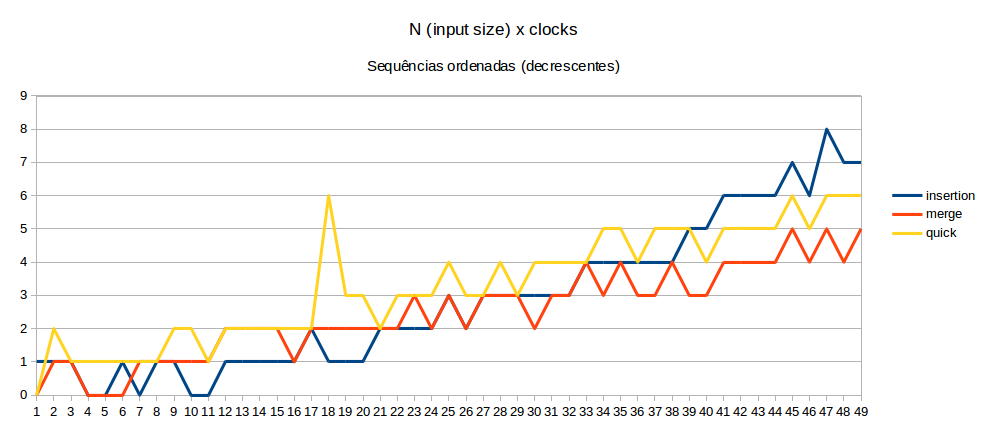
\includegraphics[width=1\textwidth]{insertion_choice}
  \end{center}
      \label{fig:k}
\end{figure}

    \paragraph{}
    Para o Merge Sort interrompemos a recursão e chamamos o Insertion Sort para N = 15. Para o Quick Sort, fizemos a mesma coisa. Além disso, para o Quick Sort, interrompemos a execução do Quick Sort para nosso N pequeno e executamos um único Insertion Sort ao final.

    \paragraph{}
    Medimos novamente o tempo para todos os tipos de entradas descritas acima (aleatórias, ordenadas crescente e decrescentemente, muitas/poucas repetições) e foi possível observar que existe ganho no desempenho ao se utilizar o Insertion Sort tanto no Merge Sort quanto no Quick Sort. 

\begin{figure}[htb]
  \begin{center}
      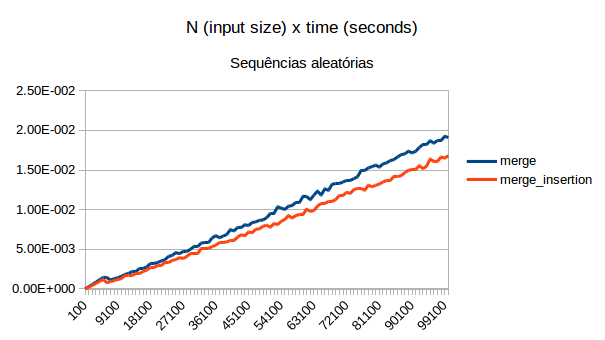
\includegraphics[width=1\textwidth,scale=0.8]{mergesort_insertion}
  \end{center}
      \label{fig:l}
\end{figure}

\begin{figure}[htb]
  \begin{center}
      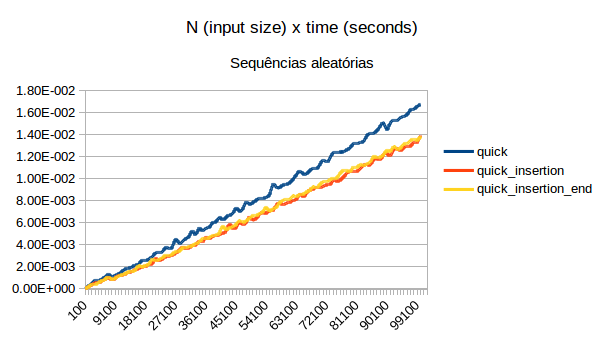
\includegraphics[width=1\textwidth]{a}
  \end{center}
      \label{fig:m}
\end{figure}

    \paragraph{}
    Ainda para o Quick Sort não ficou clara a vantagem em se fazer o Insertion Sort ao final em relação à versão executada para cada subproblema. Deixando para resolver os subproblemas no final encontramos um trade-off. Evitamos o overhead das diversas chamadas sucessivas ao Insertion Sort que teríamos que fazer para os subproblemas, mas em contrapartida, precisamos agora comparar valores previamente ordenados (desnecessariamente) pela primeira passada do Quick Sort.


    \section{Ordenando palavras}
    \paragraph{}
    Para a ordenação de palavras, a razão entre os algoritmos se manteve, porém seus tempos de execução aumentaram. Isso era esperado, dado que a ordenação de cada par de palavras implica em um número de comparações entre 1 e o número de caracteres da menor delas.
    \paragraph{}
    Por exemplo, para 100.000 inteiros o Selection Sort levava aproximadamente 13 segundos. Já para a ordenação da mesma quantidade de palavras, levou ~2.5 minutos.


\begin{table}[htb]
\centering
    \caption {BR4.txt (10.000 palavras)}
    \begin{tabular}{|c|c|}
    \toprule
    Algoritmo               & Tempo (s)\\
    \midrule
    Selection               & 1.15039  \\
    Insertion               & 0.82137  \\
    Heap                    & 0.012773 \\
    Merge                   & 0.006791 \\
    Merge + Insertion       & 0.006406 \\
    Quick                   & 0.0062   \\
    Quick + Insertion       & 0.00557  \\
    Quick + Insertion (end) & 0.005887 \\
    \bottomrule
    \end{tabular}
\end{table}

\begin{table}[htb]
\centering
    \caption {BR5.txt (100.000 palavras)}
    \begin{tabular}{|c|c|}
    \toprule
    Algoritmo               & Tempo (s)\\
    \midrule
    Selection               & 138.913  \\
    Insertion               & 100.229  \\
    Heap                    & 0.183717 \\
    Merge                   & 0.096469 \\
    Merge + Insertion       & 0.090622 \\
    Quick                   & 0.083632 \\
    Quick + Insertion       & 0.076674 \\
    Quick + Insertion (end) & 0.079223 \\
    \bottomrule
    \end{tabular}
\end{table}


\end{document}

